\chapter{Introduction}


\section{Background}

\section{Problem Statement}

A part of the computer graphics is create non-photorealistic images. A method to do this is to stylize 3D objects and 3D scenes. Stylize an object means create an image that imitates the style of an artist who would have drawn it on sheet of paper. There exist many different styles like hand drawing, brush painting, pointillism painting, stippling, watercolor painting, etc.

The main problem of stylizing a 3D object in an animation is the \textit{temporal coherence}. The \textit{temporal coherence} problem in non-photorealistic rendering encompasses both spatial and temporal aspects of the marks. The effect given by the stylization has to be kept if the object is moving, rotating and scaling. Many research has been done to solve this problem of \textit{temporal coherence} \cite{vergne_implicit_2011, benard_dynamic_2009, bleron_motion-coherent_2018}. Bénard et al. separate this problem is three sections inspired by previous work\cite{meier_painterly_1996, cunzi_dynamic_nodate, breslav_dynamic_nodate, benard_state---art_2011} the ideal solution (Figure \ref{problem_temporal_coherence} a) could correspond to something drawn by an artist at each frame. Neglect one of this three goals provide artifacts (Figure \ref{problem_temporal_coherence} b-d).

\begin{figure}
    \begin{center}
    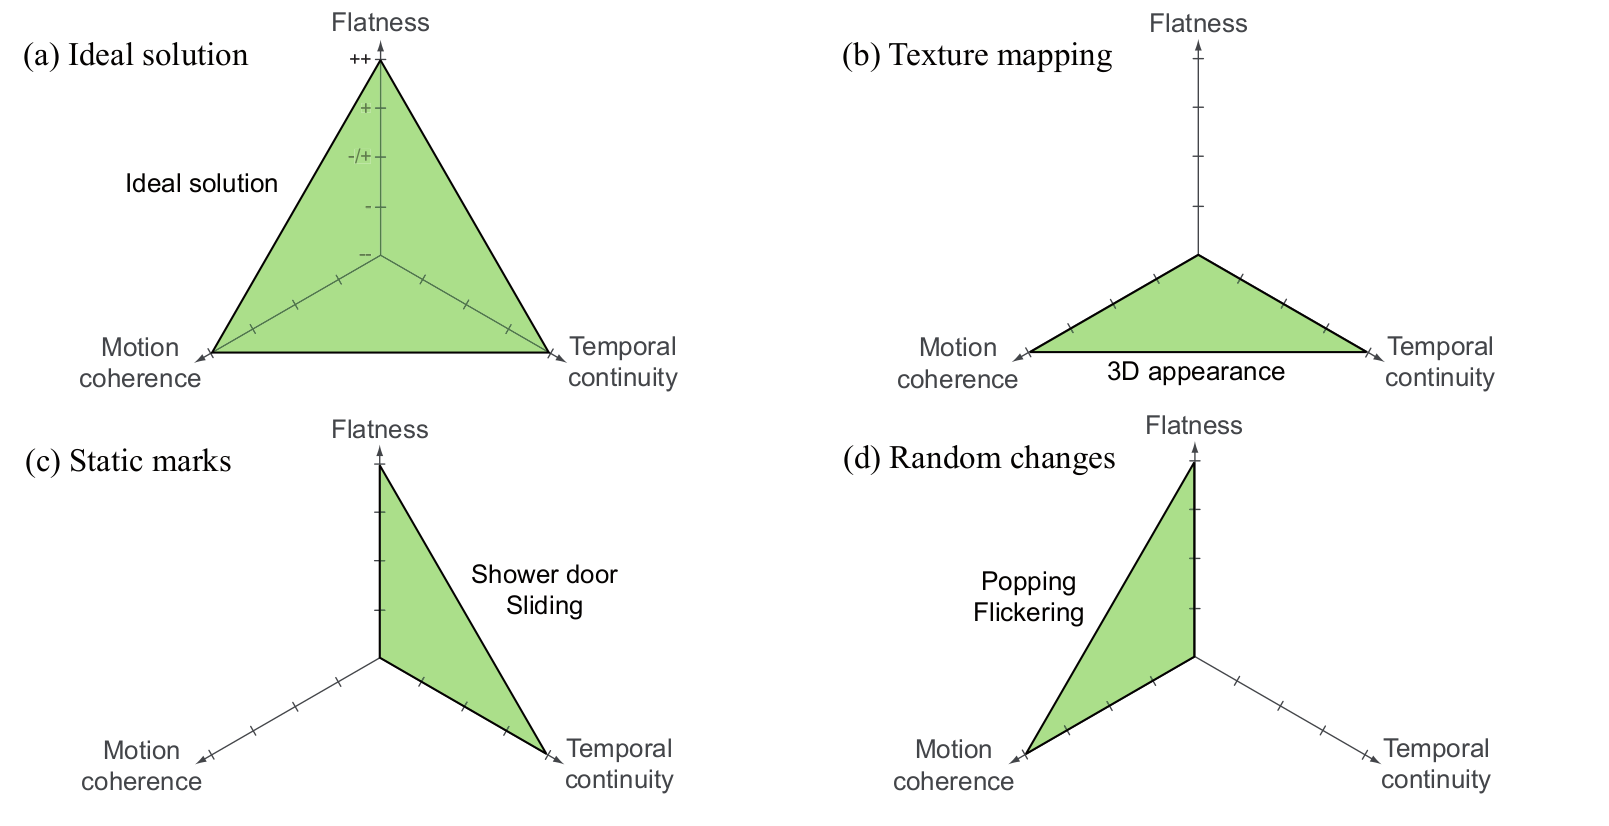
\includegraphics[scale=0.3]{pics/temporal_coherence.png}
    \end{center}
    \caption{Problem involve by temporal coherence depending of the flatness, temporal continuity, motion coherence.}
    \label{problem_temporal_coherence}
\end{figure}

\subsection{Flatness}

The impression of drawing on a flat surface gives the \textit{flatness}. The stylization has a good \textit{flatness} if the image rendered has a good 2D appearance. In order to keep this effect, the size and the distribution of the marks of your stylization have to be independent of the distance between the stylized object and the camera.

\subsection{Motion Coherence}

\textit{Motion coherence} is a correlation between the motion of marks and the motion of the 3D object. Bad \textit{Motion coherence} will give the impression to see the scene through a semi-transparent layer of marks, this is called \textit{shower door} effect \cite{meier_painterly_1996}, an example to illustrate what happens when there is a bad \textit{Motion coherence} is the movie \textit{Loving Vincent}\cite{LovingVincent}. The goal is to provide in 2D screen space a perceptual impression of motion as
close as possible to the 3D displacement in object space.

\subsection{Temporal continuity}

\textit{Temporal continuity} is the quality of minimizing changes from frame to frame to ensure fluid animations. In order to have good \textit{temporal continuity}, the marks of the image have to fade slowly during the animation. Human perception is very sensitive to \textit{temporal incoherence} according to some perceptual studies\cite{percept_studies, Schwarz_2009}. \newline


The problem introduced in the works of Bénard et al.\cite{benard_state---art_2011} is the difficulty to have a ideal solution, the one that has a good \textit{flatness}, a good \textit{motion coherence} and a good \textit{temporal continuity}. These three goals are inherently contradictory when you improve one you neglect one or maybe more. So researchers work to find solutions that make \textit{trade-offs} between these three goals. We built our approach trying to take the better of each different approach, looking at what work well and what can be integrated in our method.

\section{Scientific approach}

\section{Contents of this report}
